\documentclass[1p]{elsarticle_modified}
%\bibliographystyle{elsarticle-num}

%\usepackage[colorlinks]{hyperref}
%\usepackage{abbrmath_seonhwa} %\Abb, \Ascr, \Acal ,\Abf, \Afrak
\usepackage{amsfonts}
\usepackage{amssymb}
\usepackage{amsmath}
\usepackage{amsthm}
\usepackage{scalefnt}
\usepackage{amsbsy}
\usepackage{kotex}
\usepackage{caption}
\usepackage{subfig}
\usepackage{color}
\usepackage{graphicx}
\usepackage{xcolor} %% white, black, red, green, blue, cyan, magenta, yellow
\usepackage{float}
\usepackage{setspace}
\usepackage{hyperref}

\usepackage{tikz}
\usetikzlibrary{arrows}

\usepackage{multirow}
\usepackage{array} % fixed length table
\usepackage{hhline}

%%%%%%%%%%%%%%%%%%%%%
\makeatletter
\renewcommand*\env@matrix[1][\arraystretch]{%
	\edef\arraystretch{#1}%
	\hskip -\arraycolsep
	\let\@ifnextchar\new@ifnextchar
	\array{*\c@MaxMatrixCols c}}
\makeatother %https://tex.stackexchange.com/questions/14071/how-can-i-increase-the-line-spacing-in-a-matrix
%%%%%%%%%%%%%%%

\usepackage[normalem]{ulem}

\newcommand{\msout}[1]{\ifmmode\text{\sout{\ensuremath{#1}}}\else\sout{#1}\fi}
%SOURCE: \msout is \stkout macro in https://tex.stackexchange.com/questions/20609/strikeout-in-math-mode

\newcommand{\cancel}[1]{
	\ifmmode
	{\color{red}\msout{#1}}
	\else
	{\color{red}\sout{#1}}
	\fi
}

\newcommand{\add}[1]{
	{\color{blue}\uwave{#1}}
}

\newcommand{\replace}[2]{
	\ifmmode
	{\color{red}\msout{#1}}{\color{blue}\uwave{#2}}
	\else
	{\color{red}\sout{#1}}{\color{blue}\uwave{#2}}
	\fi
}

\newcommand{\Sol}{\mathcal{S}} %segment
\newcommand{\D}{D} %diagram
\newcommand{\A}{\mathcal{A}} %arc


%%%%%%%%%%%%%%%%%%%%%%%%%%%%%5 test

\def\sl{\operatorname{\textup{SL}}(2,\Cbb)}
\def\psl{\operatorname{\textup{PSL}}(2,\Cbb)}
\def\quan{\mkern 1mu \triangleright \mkern 1mu}

\theoremstyle{definition}
\newtheorem{thm}{Theorem}[section]
\newtheorem{prop}[thm]{Proposition}
\newtheorem{lem}[thm]{Lemma}
\newtheorem{ques}[thm]{Question}
\newtheorem{cor}[thm]{Corollary}
\newtheorem{defn}[thm]{Definition}
\newtheorem{exam}[thm]{Example}
\newtheorem{rmk}[thm]{Remark}
\newtheorem{alg}[thm]{Algorithm}

\newcommand{\I}{\sqrt{-1}}
\begin{document}

%\begin{frontmatter}
%
%\title{Boundary parabolic representations of knots up to 8 crossings}
%
%%% Group authors per affiliation:
%\author{Yunhi Cho} 
%\address{Department of Mathematics, University of Seoul, Seoul, Korea}
%\ead{yhcho@uos.ac.kr}
%
%
%\author{Seonhwa Kim} %\fnref{s_kim}}
%\address{Center for Geometry and Physics, Institute for Basic Science, Pohang, 37673, Korea}
%\ead{ryeona17@ibs.re.kr}
%
%\author{Hyuk Kim}
%\address{Department of Mathematical Sciences, Seoul National University, Seoul 08826, Korea}
%\ead{hyukkim@snu.ac.kr}
%
%\author{Seokbeom Yoon}
%\address{Department of Mathematical Sciences, Seoul National University, Seoul, 08826,  Korea}
%\ead{sbyoon15@snu.ac.kr}
%
%\begin{abstract}
%We find all boundary parabolic representation of knots up to 8 crossings.
%
%\end{abstract}
%\begin{keyword}
%    \MSC[2010] 57M25 
%\end{keyword}
%
%\end{frontmatter}

%\linenumbers
%\tableofcontents
%
\newcommand\colored[1]{\textcolor{white}{\rule[-0.35ex]{0.8em}{1.4ex}}\kern-0.8em\color{red} #1}%
%\newcommand\colored[1]{\textcolor{white}{ #1}\kern-2.17ex	\textcolor{white}{ #1}\kern-1.81ex	\textcolor{white}{ #1}\kern-2.15ex\color{red}#1	}

{\Large $\underline{12n_{0236}~(K12n_{0236})}$}

\setlength{\tabcolsep}{10pt}
\renewcommand{\arraystretch}{1.6}
\vspace{1cm}\begin{tabular}{m{100pt}>{\centering\arraybackslash}m{274pt}}
\multirow{5}{120pt}{
	\centering
	\includegraphics[width=112pt]{../../../GIT/diagram.site/Diagrams/png/2325_12n_0236.png}\\
\ \ \ A knot diagram\footnotemark}&
\allowdisplaybreaks
\textbf{Linearized knot diagam} \\
\cline{2-2}
 &
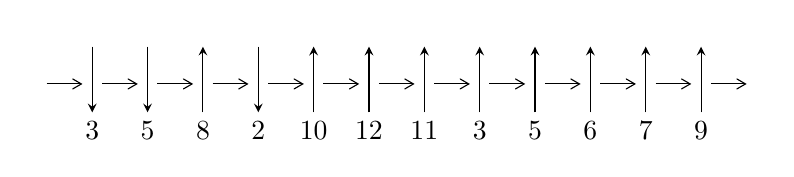
\begin{tikzpicture}[x=20pt, y=17pt]
	% nodes
	\node (C0) at (0, 0) {};
	\node (C1) at (1, 0) {};
	\node (C1U) at (1, +1) {};
	\node (C1D) at (1, -1) {3};

	\node (C2) at (2, 0) {};
	\node (C2U) at (2, +1) {};
	\node (C2D) at (2, -1) {5};

	\node (C3) at (3, 0) {};
	\node (C3U) at (3, +1) {};
	\node (C3D) at (3, -1) {8};

	\node (C4) at (4, 0) {};
	\node (C4U) at (4, +1) {};
	\node (C4D) at (4, -1) {2};

	\node (C5) at (5, 0) {};
	\node (C5U) at (5, +1) {};
	\node (C5D) at (5, -1) {10};

	\node (C6) at (6, 0) {};
	\node (C6U) at (6, +1) {};
	\node (C6D) at (6, -1) {12};

	\node (C7) at (7, 0) {};
	\node (C7U) at (7, +1) {};
	\node (C7D) at (7, -1) {11};

	\node (C8) at (8, 0) {};
	\node (C8U) at (8, +1) {};
	\node (C8D) at (8, -1) {3};

	\node (C9) at (9, 0) {};
	\node (C9U) at (9, +1) {};
	\node (C9D) at (9, -1) {5};

	\node (C10) at (10, 0) {};
	\node (C10U) at (10, +1) {};
	\node (C10D) at (10, -1) {6};

	\node (C11) at (11, 0) {};
	\node (C11U) at (11, +1) {};
	\node (C11D) at (11, -1) {7};

	\node (C12) at (12, 0) {};
	\node (C12U) at (12, +1) {};
	\node (C12D) at (12, -1) {9};
	\node (C13) at (13, 0) {};

	% arrows
	\draw[->,>={angle 60}]
	(C0) edge (C1) (C1) edge (C2) (C2) edge (C3) (C3) edge (C4) (C4) edge (C5) (C5) edge (C6) (C6) edge (C7) (C7) edge (C8) (C8) edge (C9) (C9) edge (C10) (C10) edge (C11) (C11) edge (C12) (C12) edge (C13) ;	\draw[->,>=stealth]
	(C1U) edge (C1D) (C2U) edge (C2D) (C3D) edge (C3U) (C4U) edge (C4D) (C5D) edge (C5U) (C6D) edge (C6U) (C7D) edge (C7U) (C8D) edge (C8U) (C9D) edge (C9U) (C10D) edge (C10U) (C11D) edge (C11U) (C12D) edge (C12U) ;
	\end{tikzpicture} \\
\hhline{~~} \\& 
\textbf{Solving Sequence} \\ \cline{2-2} 
 &
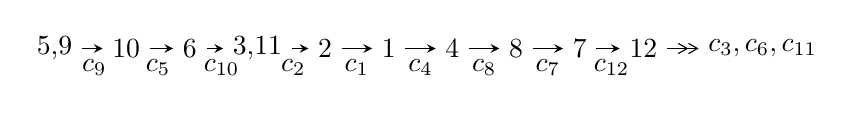
\begin{tikzpicture}[x=23pt, y=7pt]
	% node
	\node (A0) at (-1/8, 0) {5,9};
	\node (A1) at (1, 0) {10};
	\node (A2) at (2, 0) {6};
	\node (A3) at (49/16, 0) {3,11};
	\node (A4) at (33/8, 0) {2};
	\node (A5) at (41/8, 0) {1};
	\node (A6) at (49/8, 0) {4};
	\node (A7) at (57/8, 0) {8};
	\node (A8) at (65/8, 0) {7};
	\node (A9) at (73/8, 0) {12};
	\node (C1) at (1/2, -1) {$c_{9}$};
	\node (C2) at (3/2, -1) {$c_{5}$};
	\node (C3) at (5/2, -1) {$c_{10}$};
	\node (C4) at (29/8, -1) {$c_{2}$};
	\node (C5) at (37/8, -1) {$c_{1}$};
	\node (C6) at (45/8, -1) {$c_{4}$};
	\node (C7) at (53/8, -1) {$c_{8}$};
	\node (C8) at (61/8, -1) {$c_{7}$};
	\node (C9) at (69/8, -1) {$c_{12}$};
	\node (A10) at (11, 0) {$c_{3},c_{6},c_{11}$};

	% edge
	\draw[->,>=stealth]	
	(A0) edge (A1) (A1) edge (A2) (A2) edge (A3) (A3) edge (A4) (A4) edge (A5) (A5) edge (A6) (A6) edge (A7) (A7) edge (A8) (A8) edge (A9) ;
	\draw[->>,>={angle 60}]	
	(A9) edge (A10);
\end{tikzpicture} \\ 

\end{tabular} \\

\footnotetext{
The image of knot diagram is generated by the software ``\textbf{Draw programme}" developed by Andrew Bartholomew(\url{http://www.layer8.co.uk/maths/draw/index.htm\#Running-draw}), where we modified some parts for our purpose(\url{https://github.com/CATsTAILs/LinksPainter}).
}\phantom \\ \newline 
\centering \textbf{Ideals for irreducible components\footnotemark of $X_{\text{par}}$} 
 
\begin{align*}
I^u_{1}&=\langle 
8.50640\times10^{25} u^{28}+6.57905\times10^{25} u^{27}+\cdots+6.76246\times10^{26} b-3.79834\times10^{26},\\
\phantom{I^u_{1}}&\phantom{= \langle  }-8.61578\times10^{25} u^{28}-2.59629\times10^{26} u^{27}+\cdots+2.02874\times10^{27} a+4.68843\times10^{27},\\
\phantom{I^u_{1}}&\phantom{= \langle  }u^{29}+2 u^{28}+\cdots-27 u-9\rangle \\
I^u_{2}&=\langle 
b,\;- u^5+u^4+3 u^3-2 u^2+a-2 u-1,\;u^6- u^5-3 u^4+2 u^3+2 u^2+u-1\rangle \\
\\
\end{align*}
\raggedright * 2 irreducible components of $\dim_{\mathbb{C}}=0$, with total 35 representations.\\
\footnotetext{All coefficients of polynomials are rational numbers. But the coefficients are sometimes approximated in decimal forms when there is not enough margin.}
\newpage
\renewcommand{\arraystretch}{1}
\centering \section*{I. $I^u_{1}= \langle 8.51\times10^{25} u^{28}+6.58\times10^{25} u^{27}+\cdots+6.76\times10^{26} b-3.80\times10^{26},\;-8.62\times10^{25} u^{28}-2.60\times10^{26} u^{27}+\cdots+2.03\times10^{27} a+4.69\times10^{27},\;u^{29}+2 u^{28}+\cdots-27 u-9 \rangle$}
\flushleft \textbf{(i) Arc colorings}\\
\begin{tabular}{m{7pt} m{180pt} m{7pt} m{180pt} }
\flushright $a_{5}=$&$\begin{pmatrix}0\\u\end{pmatrix}$ \\
\flushright $a_{9}=$&$\begin{pmatrix}1\\0\end{pmatrix}$ \\
\flushright $a_{10}=$&$\begin{pmatrix}1\\- u^2\end{pmatrix}$ \\
\flushright $a_{6}=$&$\begin{pmatrix}u\\- u^3+u\end{pmatrix}$ \\
\flushright $a_{3}=$&$\begin{pmatrix}0.0424687 u^{28}+0.127975 u^{27}+\cdots-7.48008 u-2.31101\\-0.125788 u^{28}-0.0972878 u^{27}+\cdots+0.810929 u+0.561681\end{pmatrix}$ \\
\flushright $a_{11}=$&$\begin{pmatrix}- u^2+1\\u^4-2 u^2\end{pmatrix}$ \\
\flushright $a_{2}=$&$\begin{pmatrix}0.0424687 u^{28}+0.127975 u^{27}+\cdots-7.48008 u-2.31101\\-0.0837082 u^{28}-0.0256521 u^{27}+\cdots-0.733318 u+0.174337\end{pmatrix}$ \\
\flushright $a_{1}=$&$\begin{pmatrix}-0.207275 u^{28}-0.191732 u^{27}+\cdots+2.88280 u+0.255414\\-0.0856550 u^{28}-0.101573 u^{27}+\cdots+1.21045 u+0.659706\end{pmatrix}$ \\
\flushright $a_{4}=$&$\begin{pmatrix}0.325774 u^{28}+0.353500 u^{27}+\cdots-11.9004 u-3.50868\\-0.439150 u^{28}-0.368748 u^{27}+\cdots+6.32577 u+3.34213\end{pmatrix}$ \\
\flushright $a_{8}=$&$\begin{pmatrix}0.0733007 u^{28}+0.0609464 u^{27}+\cdots+2.08714 u-0.768665\\-0.222818 u^{28}-0.235496 u^{27}+\cdots+5.34101 u+1.86548\end{pmatrix}$ \\
\flushright $a_{7}=$&$\begin{pmatrix}0.0307540 u^{28}+0.0680917 u^{27}+\cdots+1.08829 u-0.755172\\0.00877248 u^{28}+0.0384206 u^{27}+\cdots+0.630413 u-0.299831\end{pmatrix}$ \\
\flushright $a_{12}=$&$\begin{pmatrix}-0.121620 u^{28}-0.0901590 u^{27}+\cdots+1.67234 u-0.404292\\-0.0856550 u^{28}-0.101573 u^{27}+\cdots+1.21045 u+0.659706\end{pmatrix}$\\&\end{tabular}
\flushleft \textbf{(ii) Obstruction class $= -1$}\\~\\
\flushleft \textbf{(iii) Cusp Shapes $= -\frac{119007428794930832983364079}{225415412411056701631913333} u^{28}-\frac{129789591268195455740025046}{225415412411056701631913333} u^{27}+\cdots+\frac{7277513301493536765918568604}{225415412411056701631913333} u+\frac{1889963069349290974137649138}{225415412411056701631913333}$}\\~\\
\newpage\renewcommand{\arraystretch}{1}
\flushleft \textbf{(iv) u-Polynomials at the component}\newline \\
\begin{tabular}{m{50pt}|m{274pt}}
Crossings & \hspace{64pt}u-Polynomials at each crossing \\
\hline $$\begin{aligned}c_{1}\end{aligned}$$&$\begin{aligned}
&u^{29}+39 u^{28}+\cdots+90 u+1
\end{aligned}$\\
\hline $$\begin{aligned}c_{2},c_{4}\end{aligned}$$&$\begin{aligned}
&u^{29}-7 u^{28}+\cdots-14 u+1
\end{aligned}$\\
\hline $$\begin{aligned}c_{3},c_{8}\end{aligned}$$&$\begin{aligned}
&u^{29}+u^{28}+\cdots-64 u+64
\end{aligned}$\\
\hline $$\begin{aligned}c_{5},c_{9},c_{10}\end{aligned}$$&$\begin{aligned}
&u^{29}+2 u^{28}+\cdots-27 u-9
\end{aligned}$\\
\hline $$\begin{aligned}c_{6},c_{7},c_{11}\end{aligned}$$&$\begin{aligned}
&u^{29}-2 u^{28}+\cdots+u-1
\end{aligned}$\\
\hline $$\begin{aligned}c_{12}\end{aligned}$$&$\begin{aligned}
&u^{29}+30 u^{27}+\cdots+u+1
\end{aligned}$\\
\hline
\end{tabular}\\~\\
\newpage\renewcommand{\arraystretch}{1}
\flushleft \textbf{(v) Riley Polynomials at the component}\newline \\
\begin{tabular}{m{50pt}|m{274pt}}
Crossings & \hspace{64pt}Riley Polynomials at each crossing \\
\hline $$\begin{aligned}c_{1}\end{aligned}$$&$\begin{aligned}
&y^{29}-91 y^{28}+\cdots+8066 y-1
\end{aligned}$\\
\hline $$\begin{aligned}c_{2},c_{4}\end{aligned}$$&$\begin{aligned}
&y^{29}-39 y^{28}+\cdots+90 y-1
\end{aligned}$\\
\hline $$\begin{aligned}c_{3},c_{8}\end{aligned}$$&$\begin{aligned}
&y^{29}+39 y^{28}+\cdots+49152 y-4096
\end{aligned}$\\
\hline $$\begin{aligned}c_{5},c_{9},c_{10}\end{aligned}$$&$\begin{aligned}
&y^{29}-24 y^{28}+\cdots-207 y-81
\end{aligned}$\\
\hline $$\begin{aligned}c_{6},c_{7},c_{11}\end{aligned}$$&$\begin{aligned}
&y^{29}+24 y^{28}+\cdots+y-1
\end{aligned}$\\
\hline $$\begin{aligned}c_{12}\end{aligned}$$&$\begin{aligned}
&y^{29}+60 y^{28}+\cdots+y-1
\end{aligned}$\\
\hline
\end{tabular}\\~\\
\newpage\flushleft \textbf{(vi) Complex Volumes and Cusp Shapes}
$$\begin{array}{c|c|c}  
\text{Solutions to }I^u_{1}& \I (\text{vol} + \sqrt{-1}CS) & \text{Cusp shape}\\
 \hline 
\begin{aligned}
u &= \phantom{-}0.147151 + 0.983351 I \\
a &= -0.313005 - 1.172620 I \\
b &= \phantom{-}0.619200 - 0.948695 I\end{aligned}
 & -6.51177 + 1.38864 I & -2.12482 - 1.22156 I \\ \hline\begin{aligned}
u &= \phantom{-}0.147151 - 0.983351 I \\
a &= -0.313005 + 1.172620 I \\
b &= \phantom{-}0.619200 + 0.948695 I\end{aligned}
 & -6.51177 - 1.38864 I & -2.12482 + 1.22156 I \\ \hline\begin{aligned}
u &= -1.084770 + 0.203815 I \\
a &= -0.596441 + 0.550146 I \\
b &= \phantom{-}0.210937 + 1.119990 I\end{aligned}
 & -1.04955 - 1.39392 I & \phantom{-}4.85868 + 0.24433 I \\ \hline\begin{aligned}
u &= -1.084770 - 0.203815 I \\
a &= -0.596441 - 0.550146 I \\
b &= \phantom{-}0.210937 - 1.119990 I\end{aligned}
 & -1.04955 + 1.39392 I & \phantom{-}4.85868 - 0.24433 I \\ \hline\begin{aligned}
u &= -1.11805\phantom{ +0.000000I} \\
a &= -1.24644\phantom{ +0.000000I} \\
b &= \phantom{-}1.14578\phantom{ +0.000000I}\end{aligned}
 & \phantom{-}0.572830\phantom{ +0.000000I} & \phantom{-}8.71570\phantom{ +0.000000I} \\ \hline\begin{aligned}
u &= -0.295538 + 0.824939 I \\
a &= \phantom{-}0.62455 + 1.90486 I \\
b &= -0.10295 + 1.91234 I\end{aligned}
 & -11.35050 - 1.97232 I & \phantom{-}3.18700 + 3.24359 I \\ \hline\begin{aligned}
u &= -0.295538 - 0.824939 I \\
a &= \phantom{-}0.62455 - 1.90486 I \\
b &= -0.10295 - 1.91234 I\end{aligned}
 & -11.35050 + 1.97232 I & \phantom{-}3.18700 - 3.24359 I \\ \hline\begin{aligned}
u &= -1.176090 + 0.299893 I \\
a &= \phantom{-}1.298590 + 0.500513 I \\
b &= -0.42404 + 1.73842 I\end{aligned}
 & -8.81715 - 1.90353 I & \phantom{-}3.17087 - 0.16545 I \\ \hline\begin{aligned}
u &= -1.176090 - 0.299893 I \\
a &= \phantom{-}1.298590 - 0.500513 I \\
b &= -0.42404 - 1.73842 I\end{aligned}
 & -8.81715 + 1.90353 I & \phantom{-}3.17087 + 0.16545 I \\ \hline\begin{aligned}
u &= \phantom{-}1.168350 + 0.466626 I \\
a &= \phantom{-}1.087240 - 0.320633 I \\
b &= -1.202010 - 0.277739 I\end{aligned}
 & -3.42349 + 3.73175 I & \phantom{-}3.28322 - 3.90780 I\\
 \hline 
 \end{array}$$\newpage$$\begin{array}{c|c|c}  
\text{Solutions to }I^u_{1}& \I (\text{vol} + \sqrt{-1}CS) & \text{Cusp shape}\\
 \hline 
\begin{aligned}
u &= \phantom{-}1.168350 - 0.466626 I \\
a &= \phantom{-}1.087240 + 0.320633 I \\
b &= -1.202010 + 0.277739 I\end{aligned}
 & -3.42349 - 3.73175 I & \phantom{-}3.28322 + 3.90780 I \\ \hline\begin{aligned}
u &= \phantom{-}1.252040 + 0.171380 I \\
a &= \phantom{-}0.450233 - 0.673649 I \\
b &= -0.062273 - 1.251450 I\end{aligned}
 & \phantom{-}2.49236 + 2.60548 I & \phantom{-}8.31800 - 3.45920 I \\ \hline\begin{aligned}
u &= \phantom{-}1.252040 - 0.171380 I \\
a &= \phantom{-}0.450233 + 0.673649 I \\
b &= -0.062273 + 1.251450 I\end{aligned}
 & \phantom{-}2.49236 - 2.60548 I & \phantom{-}8.31800 + 3.45920 I \\ \hline\begin{aligned}
u &= -0.340740 + 0.609315 I \\
a &= \phantom{-}0.408720 - 0.064944 I \\
b &= -0.462808 + 0.305767 I\end{aligned}
 & -3.04827 - 1.57293 I & \phantom{-}6.03185 + 4.01355 I \\ \hline\begin{aligned}
u &= -0.340740 - 0.609315 I \\
a &= \phantom{-}0.408720 + 0.064944 I \\
b &= -0.462808 - 0.305767 I\end{aligned}
 & -3.04827 + 1.57293 I & \phantom{-}6.03185 - 4.01355 I \\ \hline\begin{aligned}
u &= -1.37004 + 0.47996 I \\
a &= -0.322999 - 0.704095 I \\
b &= -0.051255 - 1.357350 I\end{aligned}
 & -1.79428 - 6.65679 I & \phantom{-}3.36940 + 5.84463 I \\ \hline\begin{aligned}
u &= -1.37004 - 0.47996 I \\
a &= -0.322999 + 0.704095 I \\
b &= -0.051255 + 1.357350 I\end{aligned}
 & -1.79428 + 6.65679 I & \phantom{-}3.36940 - 5.84463 I \\ \hline\begin{aligned}
u &= \phantom{-}0.66485 + 1.32634 I \\
a &= -0.493095 + 1.138380 I \\
b &= \phantom{-}0.22459 + 2.08826 I\end{aligned}
 & -17.4796 + 4.1704 I & -1.26801 - 2.81155 I \\ \hline\begin{aligned}
u &= \phantom{-}0.66485 - 1.32634 I \\
a &= -0.493095 - 1.138380 I \\
b &= \phantom{-}0.22459 - 2.08826 I\end{aligned}
 & -17.4796 - 4.1704 I & -1.26801 + 2.81155 I \\ \hline\begin{aligned}
u &= \phantom{-}1.47549 + 0.19394 I \\
a &= -0.329047 + 0.005572 I \\
b &= \phantom{-}0.613243 + 0.013272 I\end{aligned}
 & \phantom{-}2.92568 + 4.50321 I & \phantom{-}11.83396 - 2.97399 I\\
 \hline 
 \end{array}$$\newpage$$\begin{array}{c|c|c}  
\text{Solutions to }I^u_{1}& \I (\text{vol} + \sqrt{-1}CS) & \text{Cusp shape}\\
 \hline 
\begin{aligned}
u &= \phantom{-}1.47549 - 0.19394 I \\
a &= -0.329047 - 0.005572 I \\
b &= \phantom{-}0.613243 - 0.013272 I\end{aligned}
 & \phantom{-}2.92568 - 4.50321 I & \phantom{-}11.83396 + 2.97399 I \\ \hline\begin{aligned}
u &= -1.49199\phantom{ +0.000000I} \\
a &= \phantom{-}0.327755\phantom{ +0.000000I} \\
b &= -0.609977\phantom{ +0.000000I}\end{aligned}
 & \phantom{-}6.88521\phantom{ +0.000000I} & \phantom{-}15.7090\phantom{ +0.000000I} \\ \hline\begin{aligned}
u &= \phantom{-}1.46992 + 0.39831 I \\
a &= -1.034790 + 0.448894 I \\
b &= \phantom{-}0.52841 + 1.78278 I\end{aligned}
 & -5.70280 + 6.55116 I & \phantom{-}6.17722 - 3.52056 I \\ \hline\begin{aligned}
u &= \phantom{-}1.46992 - 0.39831 I \\
a &= -1.034790 - 0.448894 I \\
b &= \phantom{-}0.52841 - 1.78278 I\end{aligned}
 & -5.70280 - 6.55116 I & \phantom{-}6.17722 + 3.52056 I \\ \hline\begin{aligned}
u &= \phantom{-}0.395993\phantom{ +0.000000I} \\
a &= -0.267236\phantom{ +0.000000I} \\
b &= \phantom{-}0.323479\phantom{ +0.000000I}\end{aligned}
 & \phantom{-}0.588961\phantom{ +0.000000I} & \phantom{-}16.9080\phantom{ +0.000000I} \\ \hline\begin{aligned}
u &= -0.143752 + 0.301891 I \\
a &= -0.41284 - 2.66870 I \\
b &= -0.228813 - 0.666491 I\end{aligned}
 & -1.59820 - 0.73663 I & -0.70316 + 3.71220 I \\ \hline\begin{aligned}
u &= -0.143752 - 0.301891 I \\
a &= -0.41284 + 2.66870 I \\
b &= -0.228813 + 0.666491 I\end{aligned}
 & -1.59820 + 0.73663 I & -0.70316 - 3.71220 I \\ \hline\begin{aligned}
u &= -1.65985 + 0.54064 I \\
a &= \phantom{-}0.892504 + 0.457194 I \\
b &= -0.59188 + 1.84141 I\end{aligned}
 & -10.3510 - 11.0238 I & \phantom{-}2.19949 + 5.56380 I \\ \hline\begin{aligned}
u &= -1.65985 - 0.54064 I \\
a &= \phantom{-}0.892504 - 0.457194 I \\
b &= -0.59188 - 1.84141 I\end{aligned}
 & -10.3510 + 11.0238 I & \phantom{-}2.19949 - 5.56380 I\\
 \hline 
 \end{array}$$\newpage\newpage\renewcommand{\arraystretch}{1}
\centering \section*{II. $I^u_{2}= \langle b,\;- u^5+u^4+3 u^3-2 u^2+a-2 u-1,\;u^6- u^5-3 u^4+2 u^3+2 u^2+u-1 \rangle$}
\flushleft \textbf{(i) Arc colorings}\\
\begin{tabular}{m{7pt} m{180pt} m{7pt} m{180pt} }
\flushright $a_{5}=$&$\begin{pmatrix}0\\u\end{pmatrix}$ \\
\flushright $a_{9}=$&$\begin{pmatrix}1\\0\end{pmatrix}$ \\
\flushright $a_{10}=$&$\begin{pmatrix}1\\- u^2\end{pmatrix}$ \\
\flushright $a_{6}=$&$\begin{pmatrix}u\\- u^3+u\end{pmatrix}$ \\
\flushright $a_{3}=$&$\begin{pmatrix}u^5- u^4-3 u^3+2 u^2+2 u+1\\0\end{pmatrix}$ \\
\flushright $a_{11}=$&$\begin{pmatrix}- u^2+1\\u^4-2 u^2\end{pmatrix}$ \\
\flushright $a_{2}=$&$\begin{pmatrix}u^5- u^4-3 u^3+2 u^2+2 u+1\\- u\end{pmatrix}$ \\
\flushright $a_{1}=$&$\begin{pmatrix}0\\- u\end{pmatrix}$ \\
\flushright $a_{4}=$&$\begin{pmatrix}u^5- u^4-3 u^3+2 u^2+2 u+1\\0\end{pmatrix}$ \\
\flushright $a_{8}=$&$\begin{pmatrix}1\\0\end{pmatrix}$ \\
\flushright $a_{7}=$&$\begin{pmatrix}- u^5+2 u^3+u\\u^5-3 u^3+u\end{pmatrix}$ \\
\flushright $a_{12}=$&$\begin{pmatrix}u\\- u\end{pmatrix}$\\&\end{tabular}
\flushleft \textbf{(ii) Obstruction class $= 1$}\\~\\
\flushleft \textbf{(iii) Cusp Shapes $= - u^5+4 u+3$}\\~\\
\newpage\renewcommand{\arraystretch}{1}
\flushleft \textbf{(iv) u-Polynomials at the component}\newline \\
\begin{tabular}{m{50pt}|m{274pt}}
Crossings & \hspace{64pt}u-Polynomials at each crossing \\
\hline $$\begin{aligned}c_{1},c_{2}\end{aligned}$$&$\begin{aligned}
&(u-1)^6
\end{aligned}$\\
\hline $$\begin{aligned}c_{3},c_{8}\end{aligned}$$&$\begin{aligned}
&u^6
\end{aligned}$\\
\hline $$\begin{aligned}c_{4}\end{aligned}$$&$\begin{aligned}
&(u+1)^6
\end{aligned}$\\
\hline $$\begin{aligned}c_{5}\end{aligned}$$&$\begin{aligned}
&u^6+u^5-3 u^4-2 u^3+2 u^2- u-1
\end{aligned}$\\
\hline $$\begin{aligned}c_{6},c_{7}\end{aligned}$$&$\begin{aligned}
&u^6- u^5+3 u^4-2 u^3+2 u^2- u-1
\end{aligned}$\\
\hline $$\begin{aligned}c_{9},c_{10},c_{12}\end{aligned}$$&$\begin{aligned}
&u^6- u^5-3 u^4+2 u^3+2 u^2+u-1
\end{aligned}$\\
\hline $$\begin{aligned}c_{11}\end{aligned}$$&$\begin{aligned}
&u^6+u^5+3 u^4+2 u^3+2 u^2+u-1
\end{aligned}$\\
\hline
\end{tabular}\\~\\
\newpage\renewcommand{\arraystretch}{1}
\flushleft \textbf{(v) Riley Polynomials at the component}\newline \\
\begin{tabular}{m{50pt}|m{274pt}}
Crossings & \hspace{64pt}Riley Polynomials at each crossing \\
\hline $$\begin{aligned}c_{1},c_{2},c_{4}\end{aligned}$$&$\begin{aligned}
&(y-1)^6
\end{aligned}$\\
\hline $$\begin{aligned}c_{3},c_{8}\end{aligned}$$&$\begin{aligned}
&y^6
\end{aligned}$\\
\hline $$\begin{aligned}c_{5},c_{9},c_{10}\\c_{12}\end{aligned}$$&$\begin{aligned}
&y^6-7 y^5+17 y^4-16 y^3+6 y^2-5 y+1
\end{aligned}$\\
\hline $$\begin{aligned}c_{6},c_{7},c_{11}\end{aligned}$$&$\begin{aligned}
&y^6+5 y^5+9 y^4+4 y^3-6 y^2-5 y+1
\end{aligned}$\\
\hline
\end{tabular}\\~\\
\newpage\flushleft \textbf{(vi) Complex Volumes and Cusp Shapes}
$$\begin{array}{c|c|c}  
\text{Solutions to }I^u_{2}& \I (\text{vol} + \sqrt{-1}CS) & \text{Cusp shape}\\
 \hline 
\begin{aligned}
u &= -0.493180 + 0.575288 I \\
a &= -0.858925 - 1.001920 I \\
b &= \phantom{-0.000000 } 0\end{aligned}
 & -4.60518 - 1.97241 I & \phantom{-}0.92955 + 2.53106 I \\ \hline\begin{aligned}
u &= -0.493180 - 0.575288 I \\
a &= -0.858925 + 1.001920 I \\
b &= \phantom{-0.000000 } 0\end{aligned}
 & -4.60518 + 1.97241 I & \phantom{-}0.92955 - 2.53106 I \\ \hline\begin{aligned}
u &= \phantom{-}0.483672\phantom{ +0.000000I} \\
a &= \phantom{-}2.06752\phantom{ +0.000000I} \\
b &= \phantom{-0.000000 } 0\end{aligned}
 & -0.906083\phantom{ +0.000000I} & \phantom{-}4.90820\phantom{ +0.000000I} \\ \hline\begin{aligned}
u &= \phantom{-}1.52087 + 0.16310 I \\
a &= \phantom{-}0.650045 - 0.069710 I \\
b &= \phantom{-0.000000 } 0\end{aligned}
 & \phantom{-}2.05064 + 4.59213 I & \phantom{-}1.87701 - 3.61028 I \\ \hline\begin{aligned}
u &= \phantom{-}1.52087 - 0.16310 I \\
a &= \phantom{-}0.650045 + 0.069710 I \\
b &= \phantom{-0.000000 } 0\end{aligned}
 & \phantom{-}2.05064 - 4.59213 I & \phantom{-}1.87701 + 3.61028 I \\ \hline\begin{aligned}
u &= -1.53904\phantom{ +0.000000I} \\
a &= -0.649754\phantom{ +0.000000I} \\
b &= \phantom{-0.000000 } 0\end{aligned}
 & \phantom{-}6.01515\phantom{ +0.000000I} & \phantom{-}5.47870\phantom{ +0.000000I}\\
 \hline 
 \end{array}$$\newpage
\newpage\renewcommand{\arraystretch}{1}
\centering \section*{ III. u-Polynomials}
\begin{tabular}{m{50pt}|m{274pt}}
Crossings & \hspace{64pt}u-Polynomials at each crossing \\
\hline $$\begin{aligned}c_{1}\end{aligned}$$&$\begin{aligned}
&((u-1)^6)(u^{29}+39 u^{28}+\cdots+90 u+1)
\end{aligned}$\\
\hline $$\begin{aligned}c_{2}\end{aligned}$$&$\begin{aligned}
&((u-1)^6)(u^{29}-7 u^{28}+\cdots-14 u+1)
\end{aligned}$\\
\hline $$\begin{aligned}c_{3},c_{8}\end{aligned}$$&$\begin{aligned}
&u^6(u^{29}+u^{28}+\cdots-64 u+64)
\end{aligned}$\\
\hline $$\begin{aligned}c_{4}\end{aligned}$$&$\begin{aligned}
&((u+1)^6)(u^{29}-7 u^{28}+\cdots-14 u+1)
\end{aligned}$\\
\hline $$\begin{aligned}c_{5}\end{aligned}$$&$\begin{aligned}
&(u^6+u^5-3 u^4-2 u^3+2 u^2- u-1)(u^{29}+2 u^{28}+\cdots-27 u-9)
\end{aligned}$\\
\hline $$\begin{aligned}c_{6},c_{7}\end{aligned}$$&$\begin{aligned}
&(u^6- u^5+3 u^4-2 u^3+2 u^2- u-1)(u^{29}-2 u^{28}+\cdots+u-1)
\end{aligned}$\\
\hline $$\begin{aligned}c_{9},c_{10}\end{aligned}$$&$\begin{aligned}
&(u^6- u^5-3 u^4+2 u^3+2 u^2+u-1)(u^{29}+2 u^{28}+\cdots-27 u-9)
\end{aligned}$\\
\hline $$\begin{aligned}c_{11}\end{aligned}$$&$\begin{aligned}
&(u^6+u^5+3 u^4+2 u^3+2 u^2+u-1)(u^{29}-2 u^{28}+\cdots+u-1)
\end{aligned}$\\
\hline $$\begin{aligned}c_{12}\end{aligned}$$&$\begin{aligned}
&(u^6- u^5-3 u^4+2 u^3+2 u^2+u-1)(u^{29}+30 u^{27}+\cdots+u+1)
\end{aligned}$\\
\hline
\end{tabular}\newpage\renewcommand{\arraystretch}{1}
\centering \section*{ IV. Riley Polynomials}
\begin{tabular}{m{50pt}|m{274pt}}
Crossings & \hspace{64pt}Riley Polynomials at each crossing \\
\hline $$\begin{aligned}c_{1}\end{aligned}$$&$\begin{aligned}
&((y-1)^6)(y^{29}-91 y^{28}+\cdots+8066 y-1)
\end{aligned}$\\
\hline $$\begin{aligned}c_{2},c_{4}\end{aligned}$$&$\begin{aligned}
&((y-1)^6)(y^{29}-39 y^{28}+\cdots+90 y-1)
\end{aligned}$\\
\hline $$\begin{aligned}c_{3},c_{8}\end{aligned}$$&$\begin{aligned}
&y^6(y^{29}+39 y^{28}+\cdots+49152 y-4096)
\end{aligned}$\\
\hline $$\begin{aligned}c_{5},c_{9},c_{10}\end{aligned}$$&$\begin{aligned}
&(y^6-7 y^5+\cdots-5 y+1)(y^{29}-24 y^{28}+\cdots-207 y-81)
\end{aligned}$\\
\hline $$\begin{aligned}c_{6},c_{7},c_{11}\end{aligned}$$&$\begin{aligned}
&(y^6+5 y^5+\cdots-5 y+1)(y^{29}+24 y^{28}+\cdots+y-1)
\end{aligned}$\\
\hline $$\begin{aligned}c_{12}\end{aligned}$$&$\begin{aligned}
&(y^6-7 y^5+\cdots-5 y+1)(y^{29}+60 y^{28}+\cdots+y-1)
\end{aligned}$\\
\hline
\end{tabular}
\vskip 2pc
\end{document}